% ---- Präambel mit Angaben zum Dokument
\documentclass[
	fontsize=12pt,           % Leitlinien sprechen von Schriftgröße 12.
	paper=A4,
	twoside=false,
	listof=totoc,            % Tabellen- und Abbildungsverzeichnis ins Inhaltsverzeichnis
	bibliography=totoc,      % Literaturverzeichnis ins Inhaltsverzeichnis aufnehmen
	titlepage,               % Titlepage-Umgebung anstatt \maketitle
	headsepline,             % horizontale Linie unter Kolumnentitel
	abstract,              % Überschrift einschalten, Abstract muss in {abstract}-Umgebung stehen
]{scrreprt}                  % Verwendung von KOMA-Report
\usepackage[utf8]{inputenc}  % UTF8 Encoding einschalten
\usepackage[ngerman]{babel}  % Neue deutsche Rechtschreibung
\usepackage[T1]{fontenc}     % Ausgabe von westeuropäischen Zeichen (auch Umlaute)
\usepackage{microtype}       % Trennung von Wörtern wird besser umgesetzt
\usepackage{lmodern}         % Nicht-gerasterte Schriftarten (bei MikTeX erforderlich)
\usepackage{graphicx}        % Einbinden von Grafiken erlauben
\usepackage{wrapfig}         % Grafiken fließend im Text
\usepackage{setspace}        % Zeilenabstand \singlespacing, \onehalfspaceing, \doublespacing
\usepackage[
	%showframe,                % Ränder anzeigen lassen
	left=2.7cm, right=2.5cm,
	top=2.5cm,  bottom=2.5cm,
	includeheadfoot
]{geometry}                      % Seitenlayout einstellen
\usepackage{scrlayer-scrpage}    % Gestaltung von Fuß- und Kopfzeilen
\usepackage{acronym}             % Abkürzungen, Abkürzungsverzeichnis
\usepackage{titletoc}            % Anpassungen am Inhaltsverzeichnis
\contentsmargin{0.75cm}          % Abstand im Inhaltsverzeichnis zw. Punkt und Seitenzahl
\usepackage[                     % Klickbare Links (enth. auch "nameref", "url" Package)
  hidelinks,                     % Blende die "URL Boxen" aus.
  breaklinks=true                % Breche zu lange URLs am Zeilenende um
]{hyperref}
\usepackage[hypcap=true]{caption}% Anker Anpassung für Referenzen
\urlstyle{same}                  % Aktuelle Schrift auch für URLs
% Anpassung von autoref für Gleichungen (ergänzt runde Klammern) und Algorithm.
% Anstatt "Listing" kann auch z.B. "Code-Ausschnitt" verwendet werden. Dies sollte
% jedoch synchron gehalten werden mit \lstlistingname (siehe weiter unten).
\addto\extrasngerman{%
	\def\equationautorefname~#1\null{Gleichung~(#1)\null}
	\def\lstnumberautorefname{Zeile}
	\def\lstlistingautorefname{Listing}
	\def\algorithmautorefname{Algorithmus}
	% Damit einheitlich "Abschnitt 1.2[.3]" verwendet wird und nicht "Unterabschnitt 1.2.3"
	% \def\subsectionautorefname{Abschnitt}
}

% ---- Abstand verkleinern von der Überschrift 
\renewcommand*{\chapterheadstartvskip}{\vspace*{.5\baselineskip}}

% Hierdurch werden Schusterjungen und Hurenkinder vermieden, d.h. einzelne Wörter
% auf der nächsten Seite oder in einer einzigen Zeile.
% LaTeX kann diese dennoch erzeugen, falls das Layout ansonsten nicht umsetzbar ist.
% Diese Werte sind aber gute Startwerte.
\widowpenalty10000
\clubpenalty10000

% ---- Für das Quellenverzeichnis
\usepackage[
	backend = biber,                % Verweis auf biber
	language = auto,
	style = numeric,                % Nummerierung der Quellen mit Zahlen
	sorting = none,                 % none = Sortierung nach der Erscheinung im Dokument
	sortcites = true,               % Sortiert die Quellen innerhalb eines cite-Befehls
	block = space,                  % Extra Leerzeichen zwischen Blocks
	hyperref = true,                % Links sind klickbar auch in der Quelle
	%backref = true,                % Referenz, auf den Text an die zitierte Stelle
	bibencoding = auto,
	giveninits = true,              % Vornamen werden abgekürzt
	doi=false,                      % DOI nicht anzeigen
	isbn=false,                     % ISBN nicht anzeigen
    alldates=short                  % Datum immer als DD.MM.YYYY anzeigen
]{biblatex}
\addbibresource{Inhalt/literatur.bib}
\setcounter{biburlnumpenalty}{3000}     % Umbruchgrenze für Zahlen
\setcounter{biburlucpenalty}{6000}      % Umbruchgrenze für Großbuchstaben
\setcounter{biburllcpenalty}{9000}      % Umbruchgrenze für Kleinbuchstaben
\DeclareNameAlias{default}{family-given}  % Nachname vor dem Vornamen
\AtBeginBibliography{\renewcommand{\multinamedelim}{\addslash\space
}\renewcommand{\finalnamedelim}{\multinamedelim}}  % Schrägstrich zwischen den Autorennamen
\DefineBibliographyStrings{german}{
  urlseen = {Einsichtnahme:},                      % Ändern des Titels von "besucht am"
}
\usepackage[babel,german=quotes]{csquotes}         % Deutsche Anführungszeichen + Zitate


% ---- Für Mathevorlage
\usepackage{amsmath}    % Erweiterung vom Mathe-Satz
\usepackage{amssymb}    % Lädt amsfonts und weitere Symbole
\usepackage{MnSymbol}   % Für Symbole, die in amssymb nicht enthalten sind.


% ---- Für Quellcodevorlage
\usepackage{scrhack}                    % Hack zur Verw. von listings in KOMA-Script
\usepackage{listings}                   % Darstellung von Quellcode
\usepackage{xcolor}                     % Einfache Verwendung von Farben
% -- Eigene Farben für den Quellcode
\definecolor{JavaLila}{rgb}{0.4,0.1,0.4}
\definecolor{JavaGruen}{rgb}{0.3,0.5,0.4}
\definecolor{JavaBlau}{rgb}{0.0,0.0,1.0}
\definecolor{ABAPKeywordsBlue}{HTML}{6000ff}
\definecolor{ABAPCommentGrey}{HTML}{808080}
\definecolor{ABAPStringGreen}{HTML}{4da619}
\definecolor{PyKeywordsBlue}{HTML}{0000AC}
\definecolor{PyCommentGrey}{HTML}{808080}
\definecolor{PyStringGreen}{HTML}{008080}
% -- Farben für ABAP CDS
\definecolor{CDSString}{HTML}{FF8C00}
\definecolor{CDSKeywords}{HTML}{6000ff}
\definecolor{CDSAnnotation}{HTML}{00BFFF}
\definecolor{CDSComment}{HTML}{808080}
\definecolor{CDSFunc}{HTML}{FF0000}

% -- Default Listing-Styles

\lstset{
	% Das Paket "listings" kann kein UTF-8. Deswegen werden hier 
	% die häufigsten Zeichen definiert (ä,ö,ü,...)
	literate=%
		{á}{{\'a}}1 {é}{{\'e}}1 {í}{{\'i}}1 {ó}{{\'o}}1 {ú}{{\'u}}1
		{Á}{{\'A}}1 {É}{{\'E}}1 {Í}{{\'I}}1 {Ó}{{\'O}}1 {Ú}{{\'U}}1
		{à}{{\`a}}1 {è}{{\`e}}1 {ì}{{\`i}}1 {ò}{{\`o}}1 {ù}{{\`u}}1
		{À}{{\`A}}1 {È}{{\'E}}1 {Ì}{{\`I}}1 {Ò}{{\`O}}1 {Ù}{{\`U}}1
		{ä}{{\"a}}1 {ë}{{\"e}}1 {ï}{{\"i}}1 {ö}{{\"o}}1 {ü}{{\"u}}1
		{Ä}{{\"A}}1 {Ë}{{\"E}}1 {Ï}{{\"I}}1 {Ö}{{\"O}}1 {Ü}{{\"U}}1
		{â}{{\^a}}1 {ê}{{\^e}}1 {î}{{\^i}}1 {ô}{{\^o}}1 {û}{{\^u}}1
		{Â}{{\^A}}1 {Ê}{{\^E}}1 {Î}{{\^I}}1 {Ô}{{\^O}}1 {Û}{{\^U}}1
		{œ}{{\oe}}1 {Œ}{{\OE}}1 {æ}{{\ae}}1 {Æ}{{\AE}}1 {ß}{{\ss}}1
		{ű}{{\H{u}}}1 {Ű}{{\H{U}}}1 {ő}{{\H{o}}}1 {Ő}{{\H{O}}}1
		{ç}{{\c c}}1 {Ç}{{\c C}}1 {ø}{{\o}}1 {å}{{\r a}}1 {Å}{{\r A}}1
		{€}{{\euro}}1 {£}{{\pounds}}1 {«}{{\guillemotleft}}1
		{»}{{\guillemotright}}1 {ñ}{{\~n}}1 {Ñ}{{\~N}}1 {¿}{{?`}}1,
	breaklines=true,        % Breche lange Zeilen um 
	breakatwhitespace=true, % Wenn möglich, bei Leerzeichen umbrechen
	% Symbol für Zeilenumbruch einfügen
	prebreak=\raisebox{0ex}[0ex][0ex]{\ensuremath{\rhookswarrow}},
	postbreak=\raisebox{0ex}[0ex][0ex]{\ensuremath{\rcurvearrowse\space}},
	tabsize=4,                                 % Setze die Breite eines Tabs
	basicstyle=\ttfamily\small,                % Grundsätzlicher Schriftstyle
	columns=fixed,                             % Besseres Schriftbild
	numbers=left,                              % Nummerierung der Zeilen
	%frame=single,                             % Umrandung des Codes
	showstringspaces=false,                    % Keine Leerzeichen hervorheben
	keywordstyle=\color{blue},
	ndkeywordstyle=\bfseries\color{darkgray},
	identifierstyle=\color{black},
	commentstyle=\itshape\color{JavaGruen},   % Kommentare in eigener Farbe
	stringstyle=\color{JavaBlau},             % Strings in eigener Farbe,
	captionpos=b,                             % Bild*unter*schrift
	xleftmargin=5.0ex
}

% ---- Eigener JAVA-Style für den Quellcode
\renewcommand{\ttdefault}{pcr}               % Schriftart, welche auch fett beinhaltet
\lstdefinestyle{EigenerJavaStyle}{
	language=Java,                             % Syntax Highlighting für Java
	%frame=single,                             % Umrandung des Codes
	keywordstyle=\bfseries\color{JavaLila},    % Keywords in eigener Farbe und fett
	commentstyle=\itshape\color{JavaGruen},    % Kommentare in eigener Farbe und italic
	stringstyle=\color{JavaBlau}               % Strings in eigener Farbe
}

% ---- Eigener ABAP-Style für den Quellcode
\renewcommand{\ttdefault}{pcr}
\lstdefinestyle{EigenerABAPStyle}{
	language=[R/3 6.10]ABAP,
	morestring=[b]\|,                          % Für Pipe-Strings
	morestring=[b]\`,                          % für Backtick-Strings
	keywordstyle=\bfseries\color{ABAPKeywordsBlue},
	commentstyle=\itshape\color{ABAPCommentGrey},
	stringstyle=\color{ABAPStringGreen},
	tabsize=2,
	morekeywords={
		types,
		@data,
		as,
		lower,
		start,
		selection,
		order,
		by,
		inner,
		join,
		key,
		end,
		cast
	}
}

% ---- Eigener Python-Style für den Quellcode
\renewcommand{\ttdefault}{pcr}
\lstdefinestyle{EigenerPythonStyle}{
	language=Python,
	columns=flexible,
	keywordstyle=\bfseries\color{PyKeywordsBlue},
	commentstyle=\itshape\color{PyCommentGrey},
	stringstyle=\color{PyStringGreen}
}

%----- ABAP-CDS-View language
\lstdefinelanguage{ABAPCDS}{
	sensitive=false,
	%Keywords
	morekeywords={define,
		view,
		as,
		select,
		from,
		inner,
		join,
		on,
		key,
		case,
		when,
		then,
		else,
		end,
		true,
		false,
		cast,
		where,
		and,
		distinct,
		group,
		by,
		having,
		min,
		sum,
		max,
		count,
		avg
	},
	%Methoden
	morekeywords=[2]{
		div,
		currency\_conversion,
		dats\_days\_between,
		concat\_with\_space,
		dats\_add_days,
		dats\_is\_valid,
		dats\_add\_months,
		unit\_conversion,
		division,
		mod,
		abs,
		floor,
		ceil,
		round,
		concat,
		replace,
		substring,
		left,
		right,
		length
	},
	morecomment=[s][\color{CDSAnnotation}]{@}{:},
	morecomment=[l][\itshape\color{CDSComment}]{//},
	morecomment=[s][\itshape\color{CDSComment}]{/*}{*/},
	morestring=[b][\color{CDSString}]',
	keywordstyle=\bfseries\color{CDSKeywords},
	keywordstyle=[2]\color{CDSFunc}
}

  % Weitere Details sind ausgelagert

\usepackage{algorithm}                  % Für Algorithmen-Umgebung (ähnlich wie lstlistings Umgebung)
\usepackage{algpseudocode}              % Für Pseudocode. Füge "[noend]" hinzu, wenn du kein "endif",
                                        % etc. haben willst.

\makeatletter                           % Sorgt dafür, dass man @ in Namen verwenden kann.
                                        % Ansonsten gibt es in der nächsten Zeile einen Compilefehler.
\renewcommand{\ALG@name}{Algorithmus}   % Umbenennen von "Algorithm" im Header der Listings.
\makeatother                            % Zeichen wieder zurücksetzen
\renewcommand{\lstlistingname}{Listing} % Erlaubt das Umbenennen von "Listing" in anderen Titel.

% ---- Tabellen
\usepackage{booktabs}  % Für schönere Tabellen. Enthält neue Befehle wie \midrule
\usepackage{multirow}  % Mehrzeilige Tabellen
\usepackage{siunitx}   % Für SI Einheiten und das Ausrichten Nachkommastellen
\sisetup{locale=DE, range-phrase={~bis~}, output-decimal-marker={,}} % Damit ein Komma und kein Punkt verwendet wird.
\usepackage{xfrac} % Für siunitx Option "fraction-function=\sfrac"

% ---- Für Definitionsboxen in der Einleitung
\usepackage{amsthm}                     % Liefert die Grundlagen für Theoreme
\usepackage[framemethod=tikz]{mdframed} % Boxen für die Umrandung
% ---- Definition für Highlight Boxen

% ---- Grundsätzliche Definition zum Style
\newtheoremstyle{defi}
  {\topsep}         % Abstand oben
  {\topsep}         % Abstand unten
  {\normalfont}     % Schrift des Bodys
  {0pt}             % Einschub der ersten Zeile
  {\bfseries}       % Darstellung von der Schrift in der Überschrift
  {:}               % Trennzeichen zwischen Überschrift und Body
  {.5em}            % Abstand nach dem Trennzeichen zum Body Text
  {\thmname{#3}}    % Name in eckigen Klammern
\theoremstyle{defi}

% ------ Definition zum Strich vor eines Texts
\newmdtheoremenv[
  hidealllines = true,       % Rahmen komplett ausblenden
  leftline = true,           % Linie links einschalten
  innertopmargin = 0pt,      % Abstand oben
  innerbottommargin = 4pt,   % Abstand unten
  innerrightmargin = 0pt,    % Abstand rechts
  linewidth = 3pt,           % Linienbreite
  linecolor = gray!40,       % Linienfarbe
]{defStrich}{Definition}     % Name der des formats "defStrich"

% ------ Definition zum Eck-Kasten um einen Text
\newmdtheoremenv[
  hidealllines = true,
  innertopmargin = 6pt,
  linecolor = gray!40,
  singleextra={              % Eck-Markierungen für die Definition
    \draw[line width=3pt,gray!50,line cap=rect] (O|-P) -- +(1cm,0pt);
    \draw[line width=3pt,gray!50,line cap=rect] (O|-P) -- +(0pt,-1cm);
    \draw[line width=3pt,gray!50,line cap=rect] (O-|P) -- +(-1cm,0pt);
    \draw[line width=3pt,gray!50,line cap=rect] (O-|P) -- +(0pt,1cm);
  }
]{defEckKasten}{Definition}  % Name der des formats "defEckKasten"  % Weitere Details sind ausgelagert

% ---- Für Todo Notes
\usepackage{todonotes}
\setlength {\marginparwidth }{2cm}      % Abstand für Todo Notizen


% ---- Elektronische Version oder Gedruckte Version?
% ---- Unterschied: Die elektronische Version enthält keinen Platzhalter für die Unterschrift
\usepackage{ifthen}
\newboolean{e-Abgabe}
\setboolean{e-Abgabe}{false}    % false=gedruckte Fassung

% ---- Persönlichen Daten:
\newcommand{\titel}{Chess of Duty}
\newcommand{\titelheader}{Programmentwurf - Chess of Duty}
\newcommand{\arbeit}{Advanced Software-Engineering}
\newcommand{\studiengang}{Informatik}
\newcommand{\studienjahr}{2023}
\newcommand{\autor}{Clemens Richter \& Johannes Peters}
\newcommand{\autorReverse}{Richter, Clemens \& Peters, Johannes}
\newcommand{\verfassungsort}{Karlsruhe}
\newcommand{\matrikelnr}{xxxxxxx \& 5802185}
\newcommand{\kurs}{TINF20B1}
\newcommand{\bearbeitungsmonat}{April 2023}
\newcommand{\abgabe}{30. April 2023}
\newcommand{\bearbeitungszeitraum}{04.10.2022 - 30.04.2023}
\newcommand{\betreuerDhbw}{Herr Daniel Lindner}

% ---- Metainformation für das PDF Dokument
\hypersetup{
	pdftitle    = {\titel},
	pdfsubject  = {\arbeit},
	pdfauthor   = {\autor},
	%pdfkeywords = {Keywords angeben},
	pdfcreator  = {LaTeX},
	%pdfproducer = {in der Regel pdfTeX}
}

% ---- Definition der Kopf- und Fußzeilen
\clearscrheadfoot                               % Löschen von LaTeX Standard
\automark[section]{chapter}                     % Füllen von section und chapter
\renewcommand*{\chaptermarkformat}{}            % Entfernt die Kapitelnummer
\renewcommand*{\sectionmarkformat}{}            % Entfernt die Sectionnummer
% Angaben [für "plain"]{für "scrheadings"}
\ihead[]{\titelheader}                          % Kopfzeile links
\chead[]{}                                      % Kopfzeile mitte
\ohead[]{\rightmark}                            % Kopfzeile rechts
\ifoot[]{}                                      % Fußzeile links
\cfoot*{\sffamily\pagemark}                     % Fußzeile mitte
\ofoot[]{}                                      % Fußzeile rechts
\KOMAoptions{
   headsepline = 0.2pt,                         % Liniendicke Kopfzeile
   footsepline = false                          % Liniendicke Fußzeile
}

% ---- Hilfreiches
\newcommand{\zB}{z.\,B. }   % "z.B." mit kleinem Leeraum dazwischen (ohne wäre nicht korrekt)
\newcommand{\dash}{d.\,h. }

\newcommand{\code}[1]{\texttt{#1}} % Ist einfacher zu schreiben als ständig \texttt und erlaubt
                                   % Änderungen im Nachhinein, wenn man z.B. Inline-Code anders stylen möchte.

% ---- Silbentrennung (falls LaTeX defaults falsch / nicht gewünscht sind)
\hyphenation{Graph-Script} % anstatt GraphS-cript

% ---- Beginn des Dokuments
\begin{document}
\setlength{\parindent}{0pt}              % Keine Paragraphen Einrückung.
                                         % Dafür haben wir den Abstand zwischen den Paragraphen.
\setcounter{secnumdepth}{2}              % Nummerierungstiefe fürs Inhaltsverzeichnis
\setcounter{tocdepth}{1}                 % Tiefe des Inhaltsverzeichnisses. Ggf. so anpassen,
                                         % dass das Verzeichnis auf eine Seite passt.
\sffamily                                % Serifenlose Schrift verwenden.

% ---- Vorspann
% ------ Titelseite
\singlespacing
\thispagestyle{empty}
\begin{titlepage}
\enlargethispage{4cm}

\begin{figure}
	\centering
	
\includegraphics[height=5cm]{Bilder/Logos/Logo_DHBW.pdf} 
\end{figure}
		
\vspace*{0.1cm}

\begin{center}
	\huge{\textbf{\titel}}\\[1.5cm]
	\Large{\textbf{\arbeit}}\\[0.5cm]
	\normalsize{im Rahmen der Prüfung zum\\[1ex] \textbf{Bachelor of Science (B.Sc.)}}\\[0.5cm]
	\Large{des Studienganges \studiengang}\\[1ex]
	\normalsize{an der Dualen Hochschule Baden-Württemberg Karlsruhe}\\[1cm]
	\normalsize{von}\\[1ex] \Large{\textbf{\autor}} \\[1cm]
\end{center}

\vspace*{0.4cm}

\begin{center}
	%\vfill
	\begin{tabular}{ll}
		Abgabedatum:                     & \abgabe \\[0.2cm]
		Bearbeitungszeitraum:            & \bearbeitungszeitraum \\[0.2cm]
		Matrikelnummer, Kurs:            & \matrikelnr , \kurs \\[0.2cm]

		Betreuer der Arbeit:   & \betreuerDhbw \\[0.2cm]
	\end{tabular} 
\end{center}
\end{titlepage}
  % Titelseite
\newcounter{savepage}
\pagenumbering{Roman}                    % Römische Seitenzahlen
\onehalfspacing

% ------ Erklärung, Sperrvermerk, Abstact
%\include{Inhalt/01_Standard/erklaerung}
%\include{Inhalt/02_Abstract/abstract-de.tex}
%\include{Inhalt/02_Abstract/abstract-en.tex}

% ------ Inhaltsverzeichnis
\singlespacing
\tableofcontents

% ------ Verzeichnisse
\renewcommand*{\chapterpagestyle}{plain}
\pagestyle{plain}
\setcounter{savepage}{\value{page}}


% ---- Inhalt der Arbeit
\cleardoublepage
\pagenumbering{arabic}                  % Arabische Seitenzahlen für den Hauptteil
\setlength{\parskip}{0.5\baselineskip}  % Abstand zwischen Absätzen
\rmfamily
\renewcommand*{\chapterpagestyle}{scrheadings}
\pagestyle{scrheadings}
\onehalfspacing

%Hier kommen die \include-Statements
\chapter{Einleitung}

Im Rahmen des Moduls \glqq Advanced Software Engineering\grqq{} wurde ein Schachspiel als Projektgrundlage ausgewählt. 
Chess of Duty ist ein Offline-Multiplayer-Schachspiel für zwei Personen. 
Das Hauptziel des Programmentwurfs besteht darin, Schach gemäß den Standardregeln zu implementieren. 

Der Nutzen des Schachspiels für unsere Kunden entspricht dem von anderen Videospielen. 
Die Anwendung dient ausschließlich der Unterhaltung der Nutzer. 
Zusätzlich können die Anwender ihre strategischen Fähigkeiten und logisches Denken trainieren.

Das Schachspiel wird objektorientiert konzipiert und in Processing programmiert. 
Processing ist eine Open-Source-Programmiersprache, die auf Java basiert und einen besonderen Schwerpunkt auf die einfache Erstellung von Grafiken und Animationen setzt. 
Dadurch eignet sich Processing besonders für die Gestaltung interaktiver Benutzeroberflächen. 

\begin{balken}
    \tip
    \\
    Das GitHub-Repository ist mit folgendem Link erreichbar:\\
    \url{https://github.com/clemens1403/AdvSWE}
\end{balken}

\section{Vorwort}

Sehr geehrter Herr Lindner, anbei finden Sie unsere Ausarbeitung für den Programmentwurf aus dem fünften und sechsten Semester. 
Während der Projektarbeit sind verschiedene Herausforderungen aufgetreten, insbesondere bei der Projektwahl und der Auswahl des Technologiestacks. 
Für die Umsetzung einer Clean Architecture hätte sich im Nachhinein ein Verwaltungsprogramm als geeigneter erwiesen. 
Zudem gestaltete sich die Verwendung von Processing in einem Java-Projekt leider weniger intuitiv als von den Entwicklern angenommen. 
Insbesondere die Integration von Processing in IntelliJ bereitete längere Zeit Probleme.

Trotz dieser Schwierigkeiten ist das Ergebnis des Programmentwurfs ein Projekt, das die in der Vorlesung vermittelten Methoden und Prinzipien bestmöglich umsetzt. 
Sollte etwas nicht umgesetzt worden sein, wird darauf zumindest eingegangen. 

Die Implementierung der Schachlogik war äußerst umfangreich, weshalb einige Funktionen nicht unterstützt werden, beispielsweise das Schlagen en passant.
Die Durchführung eines einfachen Schachspiels ist jedoch problemlos möglich.

\section{Inbetriebnahme}

Für das Projekt, das auf GitHub einsehbar ist, wurde keine JAR-Datei erstellt. 
Das Projekt kann jedoch problemlos in IntelliJ oder Eclipse ausgeführt werden. 
Alle erforderlichen Abhängigkeiten sind in der pom-Datei des Maven-Projekts aufgeführt und im Repository verfügbar.

Es gibt eine wichtige Anmerkung, die beim Importieren der Abhängigkeiten und beim Ausführen des Projekts beachtet werden sollte. 
Abhängig von der verwendeten IDE und der Bildschirmgröße kann es vorkommen, dass Processing die Darstellung unterschiedlich skaliert, wodurch das Bild verzerrt erscheinen kann.
Dieses Problem tritt hauptsächlich bei kleinen Laptop-Bildschirmen auf, während größere Desktop-Monitore davon nicht betroffen sind.

Um das Problem zu beheben, muss in der Run-Konfiguration der Klasse \glqq Chess of Duty\grqq{} eine VM-Option angegeben werden. 
Diese Option kann ausgewählt werden, indem man auf \glqq Modify Options\grqq{} im Reiter \glqq Build and Run\grqq{} klickt und das entsprechende Feld auswählt.

\begin{minipage}{\linewidth}
    \centering
    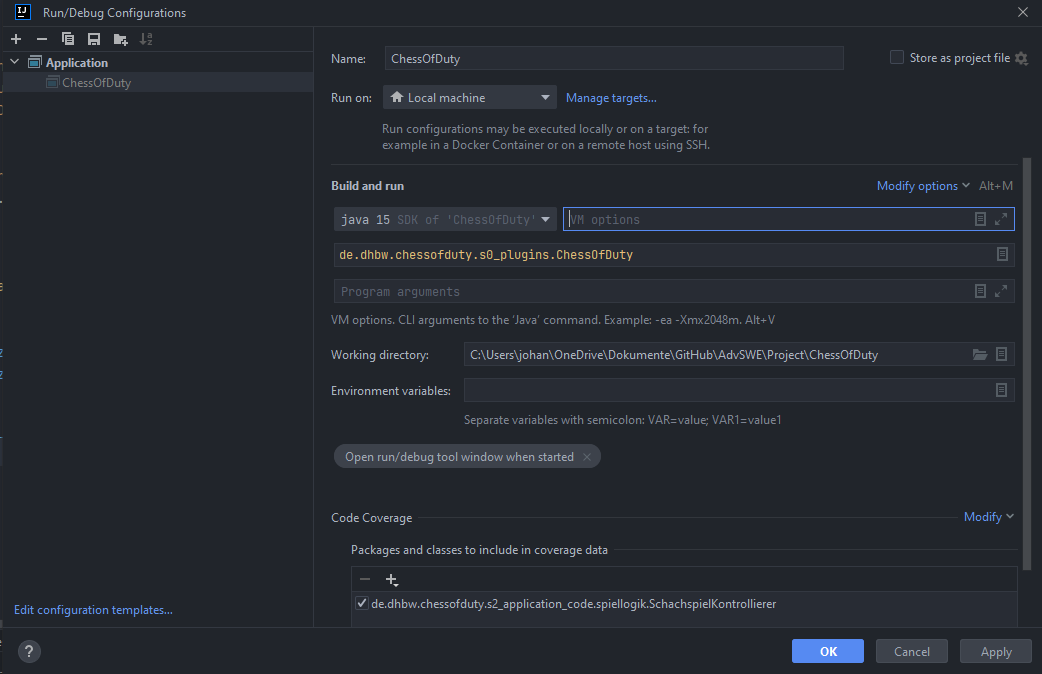
\includegraphics[scale=0.45]{Bilder/erklaerung_01.PNG}
    \captionof{figure}{Eingabefeld für VM-Options}
\end{minipage}

Sobald in das Feld Eingaben getätigt werden können, muss folgender Parameter eingetragen und gespeichert werden, bevor die Konfigurationsübersicht geschlossen und das Programm normal ausgeführt werden kann.  
\begin{figure}[h!]
    \centering
    \texttt{-Dsun.java2D.uiScale=1.0}
\end{figure}

\begin{minipage}{\linewidth}
    \centering
    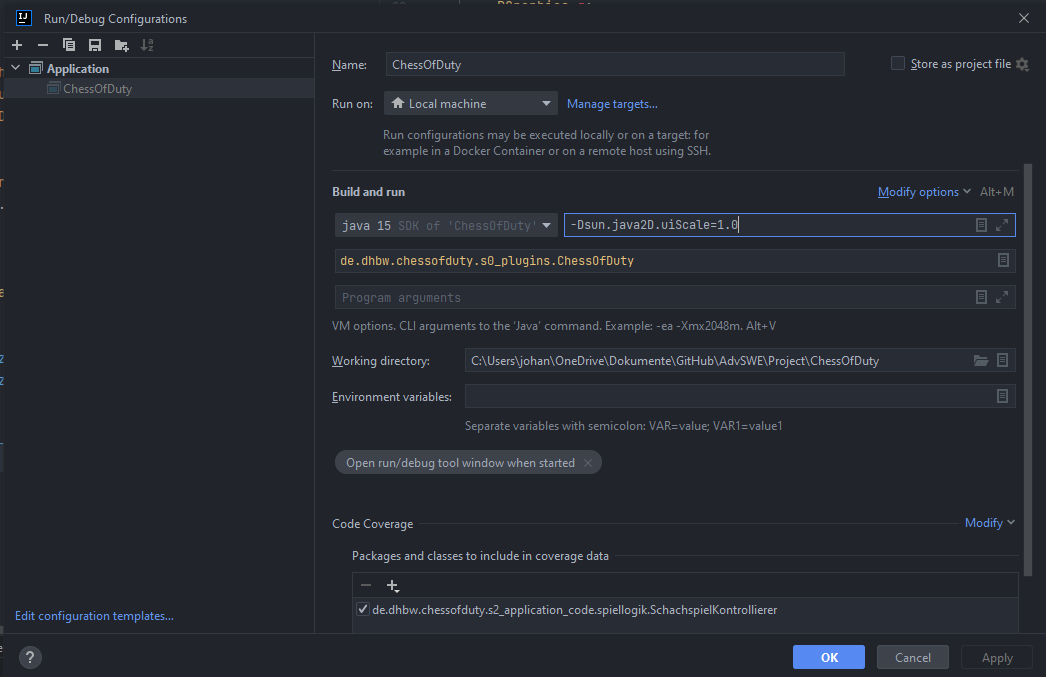
\includegraphics[scale=0.45]{Bilder/erklaerung_02.PNG}
    \captionof{figure}{VM-Options-Parameter zur richtigen Skalierung}
\end{minipage}



\chapter{Domain Driven Design}

\section{Ubiquitous Language}

Die Ubiquitous Language bezeichnet das Vokabular, welches zwischen Domänenexperten
und Entwicklern, wodurch gewährleistet werden soll, dass die gleichen Begriffe in der
Domäne und im Sourcecode verwendet werden und Missverständnisse minimiert werden.

Der Auftraggeber des Programmentwurfs ist ein deutscher Kunde. 
Obwohl in der Programmierung Englisch als die Standardsprache angenommen wird, wird aufgrund der Kundenlokalität die Projektsprache als \glqq Deutsch\grqq{} festgelegt. 
Dadurch wird versucht die meisten Ausdrücke aus der Domäne ins Deutsche zu übernehmen. 

Von der deutschen Bezeichnung ausgeschlossen sind in diesem Projekt jedoch allgemein anerkannte Java-Konventionen wie \glqq getter\grqq{} und \glqq{} setter\grqq{}. 
IDEs wie Eclipse oder Intelij sind in der Lage diese speziellen Funktionsarten automatisch zu generieren und um diese Funktion zu nutzen, werden diese Funktionsbezeichnungen auch auf Englisch akzeptiert. 
Weiterhin von der deutschen Bezeichnung ausgeschlossen sind Funktionsnamen, Objekte und Variablen, die durch die Verwendung von Processing vorgegeben sind. 
Dazu gehören beispielsweise Funktionen  wie \glqq setup(), settings()\grqq{} oder \glqq draw()\grqq{}.

\section{Domainenbausteine}

Aus der Ubiquitous Language ergeben sich nun die folgenden taktischen Muster des Domain
Driven Designs mit den entsprechenden Objekten.

\newpage

\subsection{Value Objects}

Ein Value Object repräsentiert ein bestimmtes unveränderliches Objekt, das einen bestimmten Wert besitzt und keine eigene Identität aufweist. 
Es definiert sich durch seine Eigenschaften und wird daher als austauschbar und vergleichbar angesehen.

Im Standardschach repräsentiert ein \textbf{Feld} eine Position, die durch eine Kombination aus \texttt{Spalte}, \texttt{Zeile} und \texttt{Farbe} definiert wird. 
Schachfelder haben keinen Lebenszyklus und werden aus diesem Grund als Value Objects betrachtet. 
Es ist von grundlegender Bedeutung für die Funktion eines Schachspiels, dass Schachfelder als unveränderliche Objekte behandelt werden, da ein Schachspiel auf einer \glqq festen Unterlage\grqq{} gespielt wird. 

Ein \textbf{Schachbrett} kann ebenfalls als Value Object betrachtet werden, da es einen unveränderlichen Zustand repräsentiert. 
In der domänenspezifischen Abbildung eines Schachspiels wird es als übergeordnete Verwaltungsstruktur der einzelnen Spielfelder betrachtet. 
Es besteht aus 64 Schachfeldern, die als zweidimensionale Spielebene dargestellt werden.
Die Gleichheit von zwei Schachbrettern basiert auf der Gleichheit ihrer Felder, unabhängig von ihrer tatsächlichen Instanz. 
Da die Felder als Value Objects behandelt werden und ein Schachbrett zu Beginn eines Spiels initial erzeugt und danach unverändert bleibt, wird diese Klasse auch als Value Object geführt. 
Die Integrität des Objekts muss während des Spiels gewahrt bleiben, da es keine Verhaltensänderungen aufweist. 

Ein \textbf{Schachzug} setzt sich aus einer ausgewählten \texttt{Figur}, der \texttt{Startposition}, der \texttt{Endposition} und textuellen Darstellung des Zugs zusammen.
Bei der textuellen Darstellung werden Angaben darüber, ob eine andere Figur geschlagen wird, ob durch den Zug Schach geboten wird, ob eine Bauernumwandlung stattfindet oder ob eine Rochade durchgeführt wird, berücksichtigt. 
Die Implementierung eines Schachzugs als eigene Klasse dient der Protokollierung der gespielten Schachpartie. 
Ein Schachzug wird als Value Objekt klassifiziert, da er keinen erkennbaren Lebenszyklus vorweisen kann. 
Sobald ein Spieler in einem Spiel eine Figur von Position A zu Position B bewegt, wird eine Instanz der Klasse Schachzug erstellt und kann nicht nachträglich bearbeitet werden, da auch im Spiel ein Schachzug nicht zurückgenommen oder geändert werden kann. 

\subsection{Entities}

Eine Entity ist ein Objekt, das innerhalb der Domäne eine einzigartige Identität besitzt und sich im Laufe der Zeit verändern kann. 
Entities werden durch ihre Identität und nicht durch ihre Attribute definiert und können einen Lebenszyklus vorweisen. 

Im Domainencode existiert die Klasse \textbf{Figur}, die als abstrakte Oberklasse für alle Figuren in einem Schachspiel dient. 
Da die Figur als \textit{abstract class} implementiert ist, kann sie nicht instanziiert werden. 
Aus diesem Grund wird nicht die Klasse Figur selbst, sondern alle Spielfiguren, die von Figur erben, als Entitäten zu betrachten. 
Zu diesen Spielfiguren gehören \textbf{König, Dame, Turm, Läufer, Springer} und \textbf{Bauer}.
Jede Figur kann über das Attribut \texttt{position} eindeutig identifiziert werden.
Der Schlüssel, den das genannte Attribut darstellt, ist kein natürlicher Schlüssel, da es kein wirklicher Identifikator aus der Domaine ist, sondern eine für den Betrachtungszeitpunkt eindeutige Eigenschaft der Figur. 
Da auf einem Feld im Schach immer nur eine Figur stehen kann, ist die Eindeutigkeit durch die Positionen gewährleistet. 
Wenn eine Figur auf ein Feld zieht, auf dem sich bereits eine andere Figur befindet, wird die Figur, welche ursprünglich auf dem Feld stand, geschlagen und aus dem Spiel entfernt. 
Somit steht letztendlich nur eine Figur auf dem Feld. 
Innerhalb der Domäne \glqq Schach\grqq{} ist dieser Eigenschaftsschlüssel mit jedem Schachzug veränderlich, da sich die Schachfiguren auf dem Spielfeld bewegen können. 
Die Verwendung eines Surrogatschlüssels wäre grundsätzlich auch möglich, aber in diesem Fall wird sich so gut es geht an der Domaine orientiert. 
Im analogen Schach wird der Figurentyp und die Position zur eindeutigen Identifizierung verwendet. 
Die Farbe kann indirekt durch die Anordnung der Angaben bestimmt werden.
Jede Schachfigur besitzt einen eigenen Lebenszyklus.
Sobald ein Schachspiel startet, werden alle Figuren in ihrer Startposition instanziiert.
Während des Spiels können die Figuren nahezu unbegrenzt bewegt werden. 
Wenn eine Figur geschlagen wird, wird sie wieder gelöscht. 

Obwohl ein Schachzug ein Value Object ist, wird in diesem Projekt der \textbf{Spielzug} als Entity gewertet, obwohl nur zwei Schachzüge mit einer ID zusammengefasst werden. 
Der Spielzug lässt sich eindeutig durch eine \texttt{zugNummer} identifizieren, die mit jedem Spielzug um eins inkrementiert wird.
Da diese Art der Zählung und Zugidentifizierung ebenfalls in der Domaine verwendet wird, ist die Einordnung als natürlicher Schlüssel passender als eine Bezeichnung als Surrogatschlüssel.
Der Grund, warum der Spielzug als Entity und nicht als Value Object gehandelt wird, liegt am Lebenszyklus des Objekts. 
Nach dem Erstellen einer Instanz des Spielzugs wird zuerst der Zug des Spielers \glqq Weiß\grqq{} gesetzt.
Im zweiten Schritt wird der schwarze Zug hinzugefügt, bevor der Schachzug zur Protokollierung der Schachpartie verarbeitet und final wieder verworfen wird.  

Die Klasse \textbf{Schachspiel} sollte als Entity behandelt werden, da sie eine eindeutige Identität besitzt und sich im Verlauf der Schachpartie in verschiedensten Zuständen befindet. 
Sie bildet die übergeordnete logische Ebene, welche eine bestimmte Figurenkonstellation auf dem Schachbrett zu einem bestimmten Zeitpunkt zusammenführt. 
Im Schach sind pro Zug durchschnittlich 35 unterschiedliche Züge möglich, was die Anzahl der Stellungen in einem Schachspiel exponentiell steigen lässt, abhängig von der Anzahl bereits gespielter Züge, der Positionierung der Figuren und der Anzahl der geschlagenen Figuren. 
Obwohl die Ausgangslage der Figuren immer gleich ist, unterscheidet sich die Partie Schach individuell sehr stark in ihrem Verlauf.
Um die Schachspiele eindeutig zu identifizieren, bietet sich die Verwendung eines Surrogatschlüssels an.
In der verwendeten Programmiersprache Processing, einer Java-Erweiterung, eignet sich hierfür die Verwendung einer \texttt{UUID}.

\subsection{Aggregate}

Aggregate ermöglichen die Verwaltung von Entities und Value Objects als eine zusammengehörende Einheit.
Ein Aggregat besteht dabei aus mindestens einer Entität und kann weitere Entitäten und Value Objects enthalten.

\begin{figure}[ht!]
    \centering
    \includegraphics*[scale=0.6]{Bilder/DDD_Aggregate_v2.PNG}
    \caption{Ausschnitt aus dem Domainenmodell eines Schachspiels}
\end{figure}

In der Domaine \glqq Schach\grqq{} können die Klassen \textbf{Schachbrett} und \textbf{Feld} als Aggregat zusammengefasst werden, da sie logisch miteinander verknüpft sind. 
Für ein Schachbrett werden 64 Instanzen der Klasse Feld in einer zweidimensionalen Datenstruktur gespeichert. 
Da über das Schachbrett in der Domaine die gesamte Handlung des Spiels stattfindet (Figuren werden über das Schachbrett bewegt), hat die Klasse Schachbrett eine zentrale Rolle.
Um die feste Anordnung der Felder im zweidimensionalen Rahmen des Spielfeldes durch Zeilen und Spaten positionsgetreu abzufragen, kann auf jedes Feld auf dem Schachbrett nur über das übergeordnete Schachbrett zugegriffen werden. 
Durch diese Art des Zugriffs fungiert die Klasse Schachbrett automatisch als \texttt{Root-Entity} für die Klasse Feld.
Zwischen der Root-Entität Schachbrett und der Entität Schachspiel kann die Assoziation nicht durch eine Entity-ID gelöst werden, da es sich bei dem Schachbrett um ein Value Object handelt und einem Schachbrett daher keine ID zugewiesen wird. 

Die Klasse \textbf{Spielzug} dient ebenfalls als \texttt{Root-Entity} für das Aggregat, das aus den Klassen  Spielzug und \textbf{Schachzug} besteht. 
In der Domaine kann jeder Spieler, wenn er an der Reihe ist, einen Schachzug ausführen, indem er eine Figur von Position A nach Position B bewegt. 
Ein Spielzug fasst jeweils zwei aufeinanderfolgende Schachzüge von Spieler \glqq Weiß\grqq{} und Spieler \glqq Schwarz\grqq{} zusammen. 
Die schriftliche Protokollierung einer Partie Schach erfolgt immer über die Spielzüge und gibt jeweils die einzelnen Schachzüge der unterschiedlichen Spieler an. 
Auf diese Weise kann man auf die einzelnen Schachzüge nur über die Spielzüge zugreifen, was für eine Betrachtung als Aggregat spricht.  

\subsection{Repositories}

Im Domain Driven Design werden Repositories genutzt, um Daten in einem Projekt zu persistieren und zu laden. 

Im Falle des programmierten Schachspiels soll nach jedem abgeschlossenen Spiel ein lesbares Protokoll in eine eigene Datei exportiert werden.
Obwohl die Daten nie gelesen werden, ist es erforderlich, dass für die Klasse Spielzug ein Repository verwendet wird, um die Spielzüge nacheinander in der Protokolldatei zu persistieren. 

In den Vorlesungsfolien wird beschrieben, dass meist zu jedem Aggregat auch ein entsprechendes Repository existiert. 
Für das Aggregat Schachbrett ist dies nicht der Fall. 
Das Schachbrett muss in keinem Fall persistiert werden und darum wird kein Repository benötigt. 

\subsection{Domain Service}

Ein Domain Service ist ein Konzept, das genutzt wird, um Logik abzubilden, die nicht direkt mit einer Entität oder einem Aggregat verbunden ist.

Im Schachspiel sind alle Figuren als Entitäten zu betrachten, wobei jede Figur eigene Regeln hat, nach denen sie sich auf dem Schachbrett bewegen darf.
Die Funktionalität, die die möglichen Bewegungen der verschiedenen Figurtypen ausgehend von ihrer aktuellen Position wiedergibt, befindet sich in den Klassen \textbf{Bewegungsmatrizen} und \textbf{Bewegungsrichtung}.
Beide Klassen können daher als Services in der Domaine betrachtet werden.

\chapter{Clean Architecture}
\label{txt:ca}

Das Projekt implementiert Clean Architecture durch die Verwendung von Modulen für jede Schicht. 
Dadurch wird sichergestellt, dass nur die äußeren Schichten auf die inneren Schichten zugreifen können und nicht umgekehrt. 
Die Verwendung von Schichten ermöglicht eine klare Trennung zwischen der Anwendung und der Infrastruktur, was die Wiederverwendbarkeit, Testbarkeit und Weiterentwicklung der einzelnen Komponenten erleichtert. 
Zudem ist es einfacher, einzelne Infrastrukturkomponenten auszutauschen, insbesondere je weiter sie von der Kernfunktionalität entfernt sind.

Für die Implementierung eines sauberen Schichtenmodells in einem Java-Projekt werden in der Regel separate Projekte für jede Schicht erstellt und dann in einer Entwicklungsumgebung wie IntelliJ mithilfe von Maven zusammengeführt. 
Maven kann auch verwendet werden, um Processing als festgelegten Technologiebestandteil des Projektes in IntelliJ zu integrieren. 
Allerdings stellte sich heraus, dass der Import der Processing-Dependency unzuverlässig und fehleranfällig ist. 
Um die Umsetzung der Schichtenarchitektur nicht durch ständige Maven-Installationsfehler zu behindern, wurde entschieden, die einzelnen Schichten als Packages innerhalb eines Projekts einzubinden.

Ursprünglich war das Projekt nicht in Schichten strukturiert, sondern der Code befand sich in einem einzigen Ordner, entwickelt nach dem Prinzip \glqq quick and dirty\grqq. 
Die Überarbeitung des unstrukturierten Codes und die Umstellung auf die Schichtenarchitektur erwiesen sich als komplex und zeitaufwändig.

\newpage

\section{Schicht 4 - Abstraction Code}

Diese Schicht bildet den Kern der Applikation und wird in der Regel durch die verwendete Programmiersprache repräsentiert. 
Zum Beispiel werden in Java Klassen wie \textit{String}, \textit{Boolean} oder \textit{Integer} verwendet, aber auch übergeordnete abstrakte Konzepte wie Algorithmen oder eigene Datentypen. 
Im vorliegenden Projekt konnte kein abstrakter Code identifiziert werden.
Alle mathematischen Konzepte, einschließlich der Darstellung von Bewegungsmustern einzelner Figuren, wurden als Domain Service in der dritten Schicht umgesetzt.

\section{Schicht 3 - Domain Code}

Der Domain-Code implementiert alle Bausteine der Domain, die die Quelldomäne beschreiben oder damit direkt verbunden sind und bereits im Kapitel \ref{txt:ddd} ausgearbeitet wurden. 
Diese Schicht enthält Value Objects wie \textit{Feld}, \textit{Schachbrett} und \textit{Schachzug}, die Entities \textit{Bauer}, \textit{Läufer}, \textit{Springer}, \textit{Turm}, \textit{Dame}, \textit{König} und \textit{Schachspiel}, sowie das eine Repository \textit{SpielzugRepository} und die beschriebenen Domain-Services \textit{Bewegungsmatrizen} und \textit{Bewegungsrichtung}.

\section{Schicht 2 - Application Code}

Der Application Code implementiert die gesamte Anwendungslogik des Schachspiels, die mithilfe der Domain-Bausteine die Spielfunktionen umsetzt. 
Die Anwendungsfälle des Projekts sind über Services realisiert, wobei für jede Entity und jedes Value Object ein eigener Service vorhanden ist, der die Arbeit mit diesen Elementen ermöglicht. 
Aufgrund der Verwendung der "Ubiquitous Language" in deutscher Sprache werden die Services in diesem Projekt entsprechend als "Dienst" bezeichnet.

Die in dieser Schicht implementierten Anwendungsfälle umfassen:

\begin{itemize}
    \item \textbf{Neues Schachspiel beginnen:} Um ein Spiel zu starten, wird der vorherige Spielstand, falls vorhanden, gelöscht und ein neues Spiel mit der Grundkonfiguration der Figuren initialisiert.
    \item \textbf{Schachfigur bewegen:} Jede Figur kann sich basierend auf ihrer Art (Bauer, Dame usw.) auf dem Schachbrett bewegen. 
    Abhängig von ihrer aktuellen Position werden alle möglichen Felder ermittelt, die die Figur erreichen kann. 
    Dabei werden auch die Positionen der anderen Figuren auf dem Brett berücksichtigt.
    \item \textbf{Schachfigur schlagen:} Beim Schlagen einer anderen Figur wird eine Figur bewegt, wobei dieser Anwendungsfall auf dem vorherigen aufbaut. 
    Da das Schlagen einer Figur Auswirkungen auf die im Spiel befindlichen Figuren hat, wird dies als eigener Fall betrachtet.
    \item \textbf{Schach/Schachmatt geben:} Wenn eine Figur eines Spielers ein Feld abdeckt, auf dem sich der König des anderen Spielers befindet, wird Schach geboten. 
    Ein Spieler kann den Gegenspieler durch einfaches Bewegen oder Schlagen einer anderen Figur in Schach setzen. 
    Es ist die Pflicht des Spielers, mit seinem nächsten Zug dem Schach zu entkommen. 
    Kann er dies nicht, liegt ein "Schachmatt" vor, und der Spieler, der Schach bietet, gewinnt. 
    Da das Vorhandensein von Schach oder Schachmatt den Spielverlauf entscheidend beeinflusst, handelt es sich hier um einen eigenen Anwendungsfall.
    \item \textbf{Schachzug anzeigen:} Um einen Überblick über den Spielverlauf zu erhalten, werden alle während eines Spiels ausgeführten Züge dokumentiert und übersichtlich angezeigt.
    \item \textbf{Schachspiel exportieren:} Um die Historie eines bestimmten Schachspiels zu sichern, bietet die Anwendung die Möglichkeit, den Spielverlauf in eine Datei zu exportieren. Dabei wird auf die angezeigten Züge zurückgegriffen.
\end{itemize}

Neben den Services, die die Logik der einzelnen Domain-Bausteine umsetzen, gibt es im Application Code noch die besondere Klasse \textit{Schachspielkontrollierer}. 
Diese Klasse enthält die gesamte Spiellogik, die den Ablauf des Schachspiels steuert.

\newpage

\section{Schicht 1 - Adapters}

In einem Schichtenaufbau, der Clean Architecture berücksichtigt, dienen die Adapter dazu, die Informationen und Daten aus der Domänen- und Anwendungsschicht in ein Format umzuwandeln, mit dem die visuelle Darstellung der Anwendung arbeiten kann. 
Dies beinhaltet zum Beispiel die Konvertierung verschiedener Formate. 
Da die Entities und Value Objects in der Domänenschicht bereits alle \textit{toString}-Methoden implementieren, aus denen die erforderlichen Informationen für die visuelle Darstellung abgeleitet werden können, ist in diesem Projekt keine separate Umsetzung der Adapter-Schicht erforderlich. 
Gemäß Clean Architecture müssten diese Datenbereitstellungen für die Nutzerinteraktion in die Adapter-Schicht ausgelagert werden. 
In der Praxis wären die entsprechenden Methoden jedoch in der Domänenschicht und den Adaptern sehr ähnlich, sodass ein Mapping für dieses Projekt nur zusätzliche Redundanz erzeugen würde.

\section{Schicht 0 - Plugins}

Die äußerste Schicht der Clean Architecture enthält alle extern eingebundenen Klassen, wie Frameworks und Programmschnittstellen nach außen, beispielsweise zur Persistierung von Programmdaten. 
Die Persistenz der Schachspiele ist nur in eine Richtung ausgelegt. 
In der Klasse \textit{SpielzugRepositoryBruecke} wurde die Funktion implementiert, den Verlauf eines Schachspiels in eine einfache Textdatei zu schreiben. 
Die \textit{RepositoryBruecke} ist eine Implementierung des \textit{SpielzugRepository}-Interfaces, das in der Domänenschicht liegt.

Zusätzlich zur Datenpersistenz stellt die Plugin-Schicht auch die grafische Benutzeroberfläche bereit. 
Offiziell ist Processing eine eigenständige Programmiersprache, die in Java eingebettet werden kann. 
Da Processing jedoch mit Maven in das Projekt geladen werden muss, kann man es auch als \glqq Bibliothek zum Zeichnen grafischer Komponenten\grqq{} bezeichnen. 
Die Anwendung von Processing wird ebenfalls in die Plugin-Schicht ausgelagert.

Die Hauptklasse der Benutzeroberfläche ist die Klasse \textit{Benutzeroberflaeche}.
Diese Klasse zeigt entweder einen Startbildschirm an oder lädt die Spielansicht.
In der Spielansicht werden die verschiedenen Domänenbausteine mithilfe verschiedener Zeichner-Klassen in der GUI dargestellt, die von der \textit{SchachspielZeichner-Klasse} koordiniert werden. 
Hierzu gehören die Klassen \textit{FeldZeichner}, \textit{SchachbrettZeichner} und \textit{FigurZeichner}.

\section{Dependency Inversion}

\begin{balken}
    \tip
    \\
    Commit: \\
    \footnotesize \url{https://github.com/clemens1403/AdvSWE/commit/ff87fffb24abc4050ca30019bf6800d0b60b7229}

\end{balken}

Vor der Einführung der Schichtenarchitektur bestand das Programm aus einer einzelnen Ordnerebene. 
Die Funktionen der verschiedenen Domainbausteine waren nicht in separate Schichten (Bausteine, Applikationslogik, Darstellung) aufgeteilt, sondern wurden in einer einzigen Klasse implementiert.

Processing bietet eingebaute Funktionen, die die Erstellung von Grafiken sehr einfach machen. 
Zum Beispiel gibt es die globalen Variablen \textit{mouseX} und \textit{mouseY}, die von Processing automatisch bereitgestellt werden. 
Dadurch kann die Mausposition auf der aktuellen Zeichenfläche jederzeit abgerufen werden. 
Diese Positionserfassung ist erforderlich, um Klicks auf bestimmten Elementen in der GUI zu erkennen. 
Durch die Einbindung von Processing in Java mit IntelliJ und Maven war es jedoch so, dass die von der Klasse \textit{Benutzeroberflaeche} erzeugte Zeichenfläche nur im Kontext dieser Klasse bearbeitet werden konnte. 
Daher war es nicht möglich, aus anderen Klassen auf die Mausparameter zuzugreifen. 
Um dennoch Mausklicks, z.B. bei der Auswahl eines Feldes, auswerten zu können, mussten die Mauswerte als Funktionsparameter von der \textit{Benutzeroberflaeche} an die Klassen der Domainbausteine übergeben werden.

Nachdem die Programmstruktur in Schichten aufgeteilt wurde, wurden die Repräsentation der Domainbausteine, die zugehörige Logik und die Darstellung mittels Processing voneinander entkoppelt. 
Durch die Auslagerung der Ermittlung der Zeichenparameter in die Plugin-Schicht wurde sichergestellt, dass die Prinzipien der Clean Architecture eingehalten wurden. 
Funktionen auf der Anwendungsebene, die ebenfalls die Mausparameter zur Positionsbestimmung benötigen, halten die Dependency Rule ein, indem Aufrufe nur aus der Plugin-Schicht und nicht aus der Domain-Schicht erfolgen.

Eine fachlich richtige Anwendung einer Dependency Inversion, wie sie in der Vorlesung besprochen wurde, ist die Eingrenzung von Processing auf die Zeichenebene nicht wirklich. 
In diesem Abschnitt wurde eher die Einhaltung der Dependency Rule beschrieben, doch erschien bei der Implementierung keine geeigneter Vorwand, um eine Dependency Inversion durchzuführen. 

\section{main-Methode}

Die \textit{main}-Methode einer Anwendung ist der Startpunkt für alle Aktionen, die ein Programm ausführen kann. 
Gemäß der Schichtenarchitektur befindet sich die \textit{main}-Methode \textit{ChessOfDuty} in der äußersten Schicht.
repository
\chapter{Unit Tests}
Dieses Kapitel befasst sich mit den Unit-Tests des Programmes. Dazu werden zuerst die ATRIP-Regeln erläutert und deren Anwendung beschrieben. Im Anschluss wird die Code Coverage erläutert. Zum Schluss wird noch auf die Verwendung von Mock-Objekten in den Unit-Tests eingegangen.

\section{ATRIP-Regeln}

\subsection{Automatic}
Die Regel \glqq{}Automatic\grqq{} besagt, dass die Tests ohne manuelle Eingriffe selbstständigablaufen müssen. Weiterhin müssen die Tests auch ihre Ergebnisse selbst überprüfen. Als Ergebnisse sind dabei nur \glqq{}bestanden\grqq{} oder \glqq{}nicht bestanden\grqq{} zulässig. Durch die Anwendung dieser Regel ist es möglich Unit Tests zu automatisieren.

\lstinputlisting[
	label={code:automatic},
	caption={Automatic Unit Test},
	captionpos=b,
	style=EigenerJavaStyle
]{Quellcode/automatic.java}

In Quellcode \ref{code:automatic} ist ein Unit Test aus der Klasse BauerDienstTest zu sehen. In den Zeilen 14-16 überprüft der Test mithilfe von Assertions selbst sein Ergebnis. Das eigenstädnige ablaufen des Tests wird über Maven gewährleistet. Somit ist der Test Automatic.

\subsection{Thorough}
Die Regel \glqq{}Thorough\grqq{} besagt, dass alles Notwendige getestet werden muss. Die Definition von notwendig hängt dabei immer mit den Rahmenbedingungen zusammen. Mindestens muss aber jede missionskritische Funktionalität getestet werden und für jeden aufgetretenen Fehler muss ein Testfall existieren, welcher das erneute Auftreten des Fehlers verhindert. Durch diese Regel entstehen zusätzliche Tests im Umfeld von einem Fehler, um weitere Fehler zu verhindern.

Für den konkreten Fall des Schachspiels ist es notwendig jegliche Figuren-Dienste sowie den Kontrollierer für das Schachspiel zu testen. Daher sind für alle diese Klassen Unit Tests erstellt worden. Da es sich bei dem Programm um ein Spiel handelt, ist nahezu jede Funktion die Klassen missionskritisch. Da der Aufwand für jede Methode einen Unit Test zu programmieren zu hoch für dieses Projekt wäre, wurden zu jeder Klasse ein bis zwei Unit Tests implementiert.

\subsection{Repeatable}
Die Regel \glqq{}Repeatable\grqq{} besagt, dass jeder Test automatisch durchführbar sein sollte und dabei stets das gleiche Ergebnis liefern sollte. Dazu muss der test unabhängig von der Umgebung sein. Dabei sind vor allem der Umgang mit einem Datum oder mit Zufallszahlen problematisch. Auch der Zugriff auf das Dateisystem stellt eine Abhängigkeit von der Umgebung dar.

Bei den implementierten Unit Tests gibt es keine Abhängigkeiten von der Umgebung. Die standardmäßigen Problemquellen sind für das Testen der Anwendung irrelevant, da weder Daten oder Zufallszahlen für das Testen des Schachspiels relevant sind noch ein Zugriff auf das Dateisystem in den Tests erfolgt. Das Spiel ist in sich selbst abgeschlossen, weshalb die Umgebung automatisch immer gleich ist.

\subsection{Independent}
Die Regel \glqq{}Repeatable\grqq{} besagt, dass Tests unabhängig von einander funktionieren müssen. Reihenfolge und Zusammenstellung müssen für ds ausführen der Tests irrelevant sein. Im Idealfall testet jeder Test genau einen Aspekt der zu testenden Komponente.

Da jeder Test alle benötigten Abhängigkeiten für sich selbst erzeugt erzeugt (mit zum Beispiel Mocks) gibt es keine Abhängigkeiten zu anderen Tests.

\subsection{Professional}
Die Regel \glqq{}Repeatable\grqq{} besagt, dass Testcode zum relevanten Produktionscode gehört und so leicht verständlich wie mögich sein sollte.

Um dies umzusetzen wurden zum einen sinnvolle Namen für die Testmethoden vergeben. So sind die Namen der Tests stets so aufgebaut, dass sie aus Methodenname + \glqq{}Test\grqq{} bestehen. Weiterhin sind die Tests an sich alle stets gleich aufgebaut. Zuerst werden die benötigten Abhängigkeiten erzeugt. Im Anschluss wird die zu testende Funktion ausgeführt und zum Schluss wird das Ergebnis überprüft. Durch diese Einheitliche Struktur wird für die Lesbarkeit der Tests gesorgt.  Weiterhin trägt auch eine simple Benennung von Variablen für gute Lesbarkeit.

\section{Code Coverage}
Die Code Coverage gibt an wie viel Quellcode mit Tests abgedeckt ist. Um die Code Coverage zu ermitteln kann eine Code Coverage Analyse in einer IDE ausgeführt werden. Bei Code Coverage unterschiedet man zwischen Line Coverage und Branch Coverage. Bei Line Coverage wird die Anzahl der getesten Zeilen des Quellcodes ins Verhältnis zur Gesamtzahl der Zeilen des Quellcodes gestellt. Branch Coverage hingegen beschreibt die Abdeckung von Verzweigungen im Code (if-statements). Wenn ein Test nur einen von zwei Pfaden abdeckt so liegt die Branch Coverage bei nur 50 Prozent. Bei der Code Coverage ist es wichtig dass stets angegeben wird, ob Line Coverage oder Branch Coverage verwendet wurde, da sich das Ergebnis dieser beiden Verfahren stark unterscheiden kann.

In Abbildung \ref{fig:CodeCoverage} sind die Ergebnisse einer Code Coverage Analyse für die Figuren-Dienste zu sehen. Dabei werden alle Klassen abgedeckt. Auch die Abdeckung der Methoden ist mit 94 Prozent sehr gut. Bei der Line Coverage kommen die Tests auf 59 Prozent und bei Branch Coverage nur auf 37 Prozent.
\begin{figure}[ht]
	\centering
	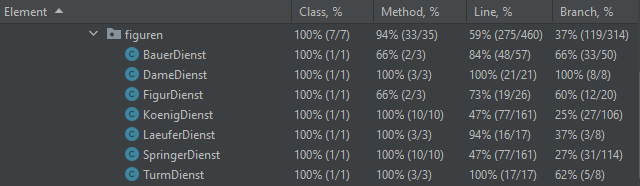
\includegraphics[width=0.8\textwidth]{Bilder/CodeCoverage.png} 
	\caption{Code Coverage-Analyse in IntelliJ für die Figuren-Dienste}
	\label{fig:CodeCoverage}
\end{figure}


\section{Mocks}
Als Mock-Objekte werden Stellvertreter für echte Objekte bezeichnet. Mithilfe dieser Stellvertreter können Abhängigkeiten bei der Durchführung von Tests ersetzt werden. Durch das ersetzen der Abhängigkeiten einer Klasse mit Mocks wird das isolierte Testen dieser Klasse möglich. Da es sehr aufwendig ist Mocks selber zu programmieren werden häufig Mock-Tools verwendet. Für den Einsatz eines Mocks muss das Mock-Objekt zuvor trainiert werden. Insgesamt durchläuft ein Mock-Objekt somit drei Phasen: Training-Phase, Einsatz-Phase und Verifikation-Phase. 

Für das Schachspiel wurde Mockito als Mock-Tool verwendet. Ein Beispiel für die Verwendung von Mocks ist in der Testklasse KoenigDienstTest zu sehen (siehe Quellcode \ref{code:Mocks} oder Github). 

\lstinputlisting[
	label={code:Mocks},
	caption={Verwendung von Mocks beim Testen},
	captionpos=b,
	style=EigenerJavaStyle
]{Quellcode/mocks.java}

In Quellcode \ref{code:Mocks} sind zwei Methoden aus der Klasse KoenigDienstTest zu sehen. Die Methode setUp (Zeile 1-8) wird vor jeder Testfunktion ausgeführt und initialisiert alle für die Tests benötigten Objekte. Unter diesen Objekten befindet sich neben einem KoenigDienst-Objekt und und einem Schachbrett-Objekt auch ein Mock-Objekt der Klasse Koenig. Das Mock-Objekt wird in Zeile 5 von Quellcode \ref{code:Mocks} erzeugt und in den Zeilen 6 und 7 eingelernt. In der Test-Methode getMoeglicheZuegeTest (Zeile 10-25 in Quellcode \ref{code:Mocks}) werden zunächst Testspezifische Mock-Objekte erzeugt. Da mit dieser Methode Interaktionen mit anderen Schachfiguren überprüft werden sollen, wird jeweils eine weiße und eine schwarze Dame als Mock-Objekt erzeugt (Zeile 12-13). In den Zeilen 14 bis 17 werden diese beiden Mock-Objekte eingelernt. Abgespielt werden die Mocks mit dem Funktionsaufruf \emph{koenigDienst.getMoeglicheZuege(figuren, schachbrett, koenigMock)} in Zeile 22. Im Anschluss wird überprüft, ob die angelernten Aufrufe mindestens ein mal genutzt wurden (Zeile 24 bis 31).
\chapter{Refactoring}
\chapter{Programming Principles}

\section{SOLID}
Die SOLID-Regeln wurden Anfang der Nullerjahre von Michael Feathers und Robert C. Martin gesammelt und formuliert. Die Regeln haben die Ziele Software wartbar, Systeme erweiterbar und Codebasen langlebiger zu machen.

\subsection{Single responsibility principle}
Das Single responsibility principle ist das Prinzip der einzigen Zuständigkeit. Somit sollte eine Klasse nur einen einzigen Grund haben sich zu ändern. Die Zuständigkeiten einer Klasse können mithilfe von Change dimensions dargestellt werden. Dabei spannt jede Zuständigkeit eine zusätzliche Achse auf. Entlang dieser Achsen werden Änderungen am Code dargestellt. Im Idealfall sind die Achsen daher orthogonal, da sich die Änderungen dadurch nicht gegenseitig beeinflussen. 

Dieses Prinzip wird im gesamten Quellcode angewendet. Die Klassen auf Domain-Ebene haben jeweils nur den Zweck das Entsprechende Objekt aus der Domain abzubilden. In der Application-Schicht hat jede Klasse Bezug zu einer Klasse aus der Domain-Ebene und nur die Aufgabe die entsprechenden Objekte zu Verwalten. Die einzige Ausnahme dabei ist der SchachspielKontrollierer, welcher die Koordination der anderen Klassen in der Application-Ebene übernimmt, um die Figuren auf dem Spielfeld miteinander interagieren zu lassen.

\subsection{Open/Closed principle}
Das Open/Closed principle besagt, dass Software-Entitäten offen für Erweiterungen sein sollen, aber gleichzeit geschlossen bezüglich Veränderungen sein sollen. Erweiterungen können zum Beispiel durch Unterklassen erschaffen werden, da nur die Unterklasse ihr Verhalten ändert, aber nicht die bereits existierende Klasse. Eine Veränderung stellt in diesem Kontext eine Modifikation des Codes durch geänderte Anforderungen dar. Zusammengefasst sollte bestehender Code also nicht mehr geändert werden müssen.

Als Beispiel für das Open/Closed principle im Code können die Figuren verwendet werden. Die Figuren sind so implementiert, dass beliebig neue Figuren hinzugefügt werden können oder Figuren ersetzt werden können.
\subsection{Liskov substitution principle}
Das LSP besagt, dass Objekte durch Instanzen ihrer Subtypen ersetzbar sein sollten, ohne die Korrektheit des Programms zu ändern. Somit gibt es strikte Regeln für Vererbungshierarchien. Subtypen dürfen dabei die Funktion der Oberklasse nicht einschränken sondern nur erweitern.

Als Beispiel für LSP können erneut die Figuren genommen werden. Zwischen der Figur-Klasse und den einzelnen Unterklassen tritt eine Kovarianz auf.


\subsection{Interface segregation principle}
Mithilfe von ISP sollen Schnittstellen mindestens in Nutzergruppen aufgeteilt werden. Dies wird umgesetzt indem anstelle eines großen Interfaces mehrere kleine Interfaces erstellt werden. Dies führt zu einer hohen Kohäsion und unterstützt auch das SRP. 

ISP wurde im Quellcode nicht angewendet, da keine Interfaces für das Spiel implementiert wurden. Die einzige sinnvolle Stelle für die verwendung eines Interfaces wäre bei den Diensten für die Figuren, da diese alle eine Methode getMoeglicheZuege implementieren. Allerdings würde dieses Interface nur eine einzelne Methode umfassen, weshalb die Anwendung von ISP hier nicht sinnvoll ist.

\subsection{Dependency inversion principle}
Das DIP besagt, dass Klassen höherer Ebenen nicht von Klassen niederer Ebe abhängig sein sollen, sondern beide im Idealfall von einem Interface abhängig sind. Dies verhindert, dass Änderungen aus einem niedrigerem Modul zu Änderungen in höheren Modulen führen. Umgesetzt wird das indem das hohe Modul eine Schnittstelle definiert, welche vom niedrigem Modul implementiert wird. Die Referenz auf die Konkrete Instanz wird dem höheren Modul dann per Dependency Injection übergeben. 

DIP wurde im Quellcode nicht angewendet. Die einzige Möglichkeit DIP anzuwenden besteht erneut bei den Figur-Diensten, welche für dieses Beispiel die niedrigeren Module darstellen. Das höhere Modul wäre der SchachspielKontrollierer. Der SchachspielKontrollierer könnte die verschiedenen Figur-Dienste als Interface definieren und die Figur-Dienste würden dann ein Interface mit der Methode getMoeglicheZuege definieren. Die Abhängigkeiten würden wie bisher per Dependency Injection übergeben werden. Jedoch wurde sich dazu entschieden dies nicht umzusetzen, da die Verständlichkeit des Codes dadurch sinkt (unserem empfinden nach). Durch die klare Typisierung der verschiedenen Figur-Dienste ist der Code strukturierter und man kann zusätzlich zum Name der Variable auch Anhand des Typs erkennen, welche Aufgabe der entsprechende Dienst hat.

\section{GRASP}
GRASP steht für General Responsibility Assignment Software Patterns/Principles und stellt Standardlösungen für Typische Fragestellungen bei der Softwareentwicklung dar. Insgesamt stellt GRASP neun Prinzipien/Werkzeuge bereit:
\begin{itemize}
    \item Low Coupling
    \item High Cohesion
    \item Indirection
    \item Polymorphism
    \item Pure Fabrication
    \item Controller
    \item Information Expert
    \item Creator
\end{itemize}

In den folgenden Abschnitten wird kurz das Konzept der Kopplung und das Konzept der Kohäsion erläutert und die Anwendung im Quellcode beschrieben.

\subsection{Kopplung}
Als Kopplung wird das Maß für die Abhängigkeit einer Klasse von ihrer Umgebung bezeichnet. Durch geringe Kopplung werden viele Vorteile ermöglicht. So lässt sich Code mit geringer Kopplung leicht anpassen und gut Testen. Weiterhin ist der Code leichter verständlich und kann besser wiederverwendet werden.

Der Quellcode ist eher ein negativ-Beispiel für geringe Kopplung. Dies kann daran erkannt werden, dass zum größten Teil statische Methodenaufrufe ausgeführt werden, keine Interfaces verwendet werden bis auf den Beobachter, und auch keine Events auf einem Eventbus versendet werden. Als größtes Negativ-Beispiel im Quellcode kann man den Schachspielkontrollierer nehmen, welcher an eine Vielzahl von anderen Klassen und Methoden gekoppelt ist.

\subsection{Kohäsion}
Bei Kohäsion handelt es sich um das Maß für den inneren Zusammenhalt einer Klasse. Dabei ist Kohäsion ein semantisches Maß - also abhängig von der menschlichen Einschätzung.

Die Kohäsion des Quellcodes ist relativ hoch. In den Klassen der Figur-Dienste rufen sich die Methoden zum größten Teil untereinander auf. Die Klassen der Figuren-Dienste können allgemein als positives Beispiel für eine hohe Kohäsion genommen werden.


\section{DRY}

DRY steht für Don't Repeat Yourself und besagt, dass man alles einmal machen soll und nur einmal machen soll. Das Motto von Dry ist kann wiefolgt definiert werden: \glqq{} Jeder Wissensaspekt darf nur eine einzige, nicht zweideutige verbindliche Repräsentation in einem System besitzen\grqq{}. Mechanische Duplikation ist dabei jedoch erlaubt, solange die Originalquelle klar definiert ist. Somit ändert eine Modifikation alle verknüpften Elemente in gleicher Weise, aber ändert keine nicht verknüpften Elemente.

Im Quellcode ist dieses Prinzip zum Beispiel in der Klasse SpringerDienst zu erkennen. Die Klasse definiert wiederverwendbare und universell anwendbare Methoden ohne sich zu wiederholen.

% ---- Literaturverzeichnis
\cleardoublepage
\renewcommand*{\chapterpagestyle}{plain}
\pagestyle{plain}
\pagenumbering{Roman}                   % Römische Seitenzahlen
\setcounter{page}{\numexpr\value{savepage}+1}

% ---- Anhang
\appendix
%\clearpage
%\pagenumbering{Roman}  % römische Seitenzahlen für Anhang

\newpage
\end{document}